\documentclass{beamer}
\usepackage[utf8]{inputenc}
\usepackage[T1]{fontenc}
%\usepackage[french]{babel}
\usepackage{amsmath, amsfonts, amsthm, amssymb}
\usepackage{hyperref}
\usepackage{tcolorbox}
\usepackage{sagetex}
\usepackage{fancyvrb}

\usetheme{default}


\title{Sage\TeX ~tutorial}
\author{Pauline Hubert}
\date{FPSAC software days, July 2019}

\begin{document}
	\maketitle
	
	\begin{frame}{Why use Sage\TeX ?}
	Sage\TeX~ is a Sage package that allows you to add Sage code and run it directly in a \LaTeX~ document. \newline \pause
	
	\begin{itemize}
		\item Print Sage code
		\item Print the result of Sage commands without having to copy and paste
		\item Plot graphs
		\item Generate multiple versions of the same document
	\end{itemize}
	\end{frame}

	\begin{frame}[fragile]{How to use it?}
		\begin{enumerate}
			\item Copy the file \texttt{sage.sty} in your working directory. 
			
			This file can be found at 
			\begin{verbatim}
				$SAGE_ROOT/local/share/texmf/tex/latex/sagetex
			\end{verbatim}
			where \texttt{\$SAGE\_ROOT} is where you installed sage on your computer.
			%Add link
			%/home/pauline/texmf/tex/latex
			\item Add the package \texttt{sagetex} in your tex file.
			\item Add SageTex commands in your latex.
			\item Compile normally. This will generate a \texttt{.sagetex.sage} file. 
			\item Execute this file in a terminal.
			\begin{verbatim}
			sage FILE_NAME.sagetex.sage
			\end{verbatim}
			\item Compile your latex once again. 
			 
		\end{enumerate}
	\end{frame}

	\begin{frame}[fragile]{Inline Sage}
		Include a Sage output in the text in maths mode. \newline
		
		What I write:
		\begin{Verbatim}[frame=single]
This is an example $2+2 = \sage{2+2}$.
The integer $150$ admits 
$\sage{number_of_partitions(150)}$ partitions.
		\end{Verbatim}

		\vspace{.5cm}
		
		What I get: 
		
		\fbox{\parbox{\textwidth}{
		This is an example $2+2 = \sage{2+2}$.
		
		The integer $150$ admits $\sage{number_of_partitions(150)}$ partitions.}}
		
	\end{frame}

	\begin{frame}[fragile]{Sage block}
	You can print some sage code using \texttt{sageblock}. \newline
	
	I can write
	\begin{Verbatim}[frame=single]
\begin{sageblock}
	f(x) = exp(x) * sin(2*x)
\end{sageblock}
	\end{Verbatim}
	
	And I get : 
	
	\begin{sageblock}
		f(x) = exp(x) * sin(2*x)
	\end{sageblock}
		
	\end{frame}
	\begin{frame}[fragile]{Sage commandline}
		If you want to print Sage code and its output use \texttt{sagecommandline}. \newline 
		
		What I write
		\begin{Verbatim}[frame=single]
\begin{sagecommandline}
	sage: 1+1
	sage: is_prime(57)
	sage: if is_prime(57):
	....:     print('prime')
	....: else:
	....:     print('composite')
\end{sagecommandline}
		\end{Verbatim}	
	
	\end{frame}
	\begin{frame}[fragile]{Sage commandline}
		If you want to print Sage code and its output use \texttt{sagecommandline}. \newline 
				
		What I get
		
		\begin{sagecommandline}
			sage: 1+1
			sage: is_prime(57)
			sage: if is_prime(57):
			....:     print('prime')
			....: else:
			....:     print('composite')
		\end{sagecommandline}	
		
		\end{frame}
	\begin{frame}[fragile]{Sage silent}
		You may want to run some Sage commands but without printing them in the text. This is what \texttt{sagesilent} does. \newline
		
		I can write : \newline
		
		\begin{Verbatim}[frame=single]
\begin{sagesilent}
	var('x,y')
	M = matrix([[i+j for i in range(3)] 
			for j in range(3)])
\end{sagesilent}

And later in the text you may want to define 
the matrix $M$ as 
$$M:= \sage{M}$$
and print its determinant which is 
$\sage{M.determinant()}$.
		\end{Verbatim}
	
	\end{frame}
	\begin{frame}[fragile]{Sage silent}
		You may want to run some Sage commands but without printing them in the text. This is what \texttt{sagesilent} does. \newline
		
		\begin{sagesilent}
			var('x,y')
			M = matrix([[i+j for i in range(3)] for j in range(3)])
		\end{sagesilent}
	
		And I get : \newline
		
		\fbox{
		\begin{minipage}{\textwidth}
		And later in the text you may want to define the matrix $M$ as $$M:= \sage{M}$$
		and print its determinant which is $\sage{M.determinant()}$.
		\end{minipage}}

	\end{frame}
	\begin{frame}[fragile]{Sage plot}
	You can also use SageTex commands to plot functions and graphs. 
		\begin{Verbatim}[frame=single]
\begin{center}
	\sageplot[height=5cm]{plot(f, -1, 1)}
\end{center}
		\end{Verbatim}
		
		\begin{center}\sageplot[height=5cm]{plot(f, -1, 1)}\end{center}
		
	\end{frame}
	\begin{frame}[fragile]{Sage plot}
	You can also use SageTex commands to plot functions and graphs. \newline 
	 
	\begin{Verbatim}[frame=single]
\begin{sagesilent}
	G = graphs.PetersenGraph()
	c = G.coloring(hex_colors=True)
\end{sagesilent}

Let's print the Petersen graph.
\begin{center}
\sageplot[height=5cm]{G.plot(vertex_labels=False, 
	vertex_size=400)}
\end{center}
	\end{Verbatim}	
	\end{frame}
	\begin{frame}[fragile]{Sage plot}
		You can also use SageTex commands to plot functions and graphs. \newline
		
		\begin{sagesilent}
			G = graphs.PetersenGraph()
			c = G.coloring(hex_colors=True)
		\end{sagesilent}

		Let's print the Petersen graph.
		\begin{center}
			\sageplot[height=5cm]{G.plot(vertex_labels=False, vertex_size=400)}
		\end{center}
	
	\end{frame}
	\begin{frame}{Automatically generated files}
		You can also combine Latex and Sage features. For example ramdom matrices in Sage and file generating commands in Latex, can be combined to automatically obtain several versions of the same homework. \newline
		
		\footnotesize{From Aram's website}
		\begin{figure}[h]
			\centering
			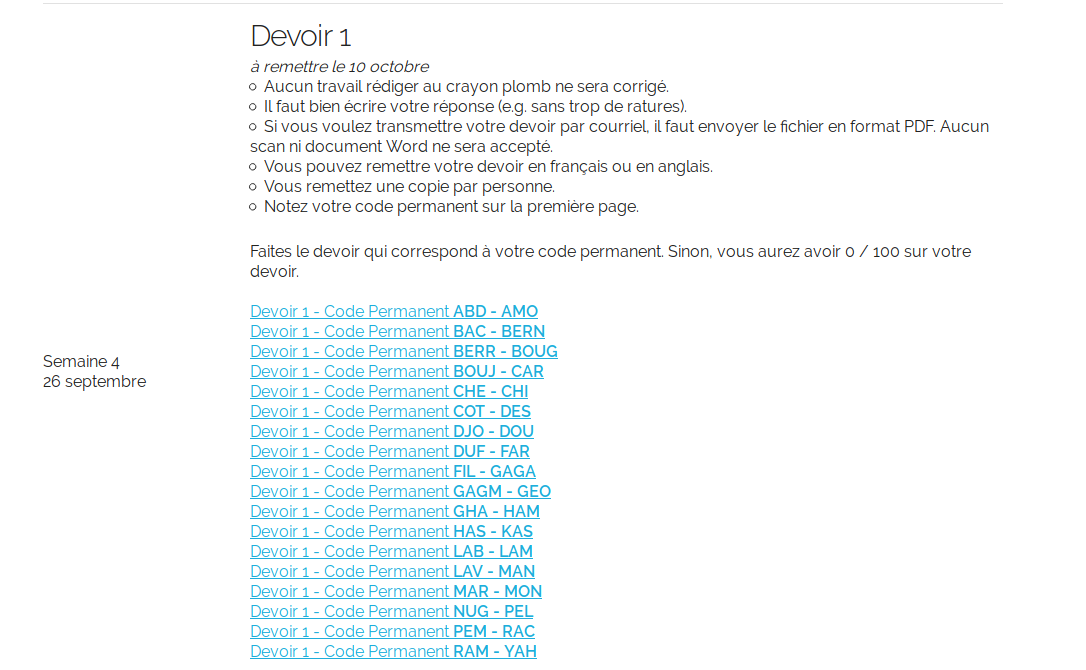
\includegraphics[scale=.2]{img1.png}
		\end{figure}
		
	\end{frame}
	\begin{frame}{Automatically generated files}
	You can also combine Latex and Sage features. For example ramdom matrices in Sage and file generating commands in Latex, can be combined to automatically obtain several versions of the same homework. \newline
	
	\footnotesize{For Aram's website}
	\begin{figure}[h]
		\centering
		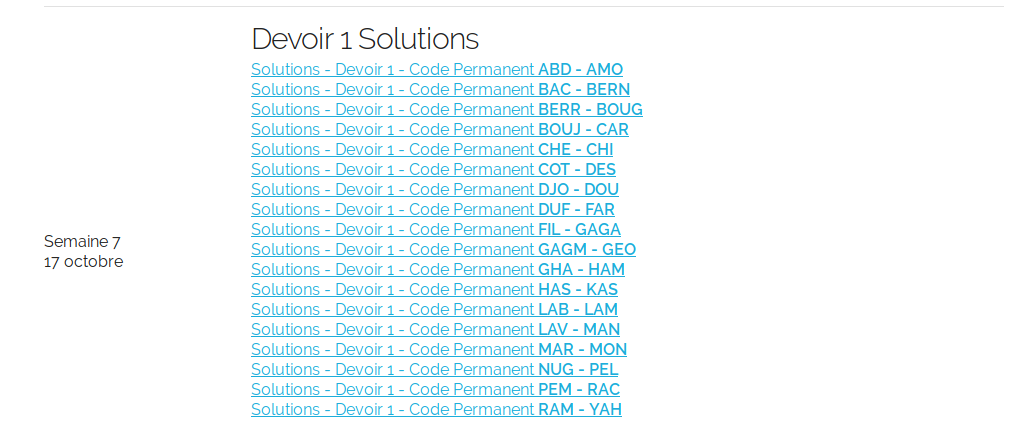
\includegraphics[scale=.2]{img2.png}
	\end{figure}
	
	\end{frame}
	\begin{frame}{Conclusion}
	
	{\Large Some references}
	\begin{thebibliography}{99}
		\bibitem{documentation} Sage\TeX ~documentation \url{http://ctan.ijs.si/tex-archive/macros/latex/contrib/sagetex/sagetex.pdf}
		\bibitem{example} A nice example\\ \url{https://github.com/sagemath/sagetex}
		\bibitem{nadia} Nadia's notes on Sage\TeX ~(french) \url{https://nadialafreniere.github.io/sage}
		\bibitem{slides} \href{https://phubert.github.io/sage.html}{Slides}
	\end{thebibliography}
	\end{frame}

\end{document}